% =============================================================================
%  Diplomado en Data Science Aplicada con Python para la Toma de Decisiones
%  Clase 8: Conoce tus Datos — Estructura, Tipos y Limpieza
%  Arca Continental Ecuador | UDLA
%
%  Compilar: pdflatex -shell-escape presentacion.tex (x2 para refs)
% =============================================================================
\documentclass[aspectratio=169, 11pt]{beamer}

\usepackage[T1]{fontenc}
\usepackage[utf8]{inputenc}
\usepackage[spanish,es-noshorthands]{babel}
\usepackage{FiraSans}
\usepackage{FiraMono}
\renewcommand{\familydefault}{\sfdefault}
\usepackage{graphicx}
\usepackage{tikz}
\usetikzlibrary{arrows.meta, positioning, shapes.geometric, shapes.misc,
  calc, fit, decorations.pathreplacing, backgrounds}
\usepackage{fontawesome5}
\usepackage{minted}
\usepackage{tcolorbox}
\tcbuselibrary{minted, skins, breakable}
\usepackage{booktabs}
\usepackage{colortbl}
\usepackage{multicol}
\usepackage{hyperref}
\usepackage{calc}

\definecolor{arcaRed}{HTML}{C82B40}
\definecolor{arcaDark}{HTML}{6B1525}
\definecolor{udlaCrimson}{HTML}{A31545}
\definecolor{arcaGray}{HTML}{F5F5F5}
\definecolor{arcaLightGray}{HTML}{EBEBEB}
\definecolor{textDark}{HTML}{2D2D2D}
\definecolor{textMuted}{HTML}{6B7280}
\definecolor{codeGreen}{HTML}{16A34A}
\definecolor{codeBlue}{HTML}{2563EB}
\definecolor{codeOrange}{HTML}{EA580C}
\definecolor{dikwData}{HTML}{94A3B8}
\definecolor{dikwInfo}{HTML}{2563EB}
\definecolor{dikwKnow}{HTML}{7C3AED}
\definecolor{dikwWis}{HTML}{C82B40}
\definecolor{beerYellow}{HTML}{F59E0B}
\definecolor{beerPink}{HTML}{EC4899}

\usetheme{default}
\usecolortheme{default}
\setbeamertemplate{navigation symbols}{}
\setbeamertemplate{footline}{}
\setbeamertemplate{headline}{}
\setbeamercolor{normal text}{fg=textDark}
\setbeamercolor{frametitle}{fg=arcaRed, bg=white}
\setbeamercolor{title}{fg=white}
\setbeamercolor{subtitle}{fg=white!85}
\setbeamercolor{author}{fg=white!80}
\setbeamercolor{date}{fg=white!70}
\setbeamercolor{item}{fg=arcaRed}
\setbeamercolor{subitem}{fg=arcaDark}
\setbeamercolor{block title}{fg=white, bg=arcaRed}
\setbeamercolor{block body}{fg=textDark, bg=arcaGray}
\setbeamercolor{block title alerted}{fg=white, bg=codeOrange}
\setbeamercolor{block body alerted}{fg=textDark, bg=arcaGray}
\setbeamercolor{block title example}{fg=white, bg=codeGreen}
\setbeamercolor{block body example}{fg=textDark, bg=arcaGray}
\setbeamercolor{section in toc}{fg=arcaDark}
\setbeamerfont{frametitle}{size=\Large, series=\bfseries}
\setbeamerfont{title}{size=\huge, series=\bfseries}
\setbeamerfont{subtitle}{size=\large}
\setbeamerfont{author}{size=\normalsize}
\setbeamerfont{date}{size=\small}
\setbeamerfont{block title}{size=\normalsize, series=\bfseries}
\setbeamerfont{footnote}{size=\tiny}
\setbeamertemplate{itemize item}{\scriptsize\raise1.5pt\hbox{\color{arcaRed}$\blacktriangleright$}}
\setbeamertemplate{itemize subitem}{\scriptsize\raise1pt\hbox{\color{arcaDark}$\bullet$}}
\setbeamertemplate{enumerate items}[default]
\setbeamercolor{enumerate item}{fg=arcaRed}

\setbeamertemplate{headline}{%
  \begin{tikzpicture}[remember picture, overlay]
    \fill[arcaDark] (current page.north west) rectangle
      ([yshift=-0.7cm]current page.north east);
    \node[anchor=west, inner sep=0pt] at
      ([xshift=0.6cm, yshift=-0.35cm]current page.north west)
      {
\includegraphics[height=0.45cm]{../logo_udla_white.png}};
    \node[anchor=east, inner sep=0pt] at
      ([xshift=-0.6cm, yshift=-0.35cm]current page.north east)
      {
\includegraphics[height=0.45cm]{../ArcaContinental_white.png}};
  \end{tikzpicture}%
  \vspace{0.7cm}%
}

\setbeamertemplate{footline}{%
  \begin{tikzpicture}[remember picture, overlay]
    \draw[arcaLightGray, line width=0.4pt]
      ([yshift=0.35cm, xshift=0.6cm]current page.south west) --
      ([yshift=0.35cm, xshift=-0.6cm]current page.south east);
    \node[anchor=south, font=\tiny\color{textMuted}] at
      ([yshift=0.08cm]current page.south)
      {Diplomado en Data Science Aplicada con Python \(\cdot\) Arca Continental Ecuador};
    \node[anchor=south east, font=\scriptsize\bfseries\color{arcaRed}] at
      ([xshift=-0.6cm, yshift=0.08cm]current page.south east)
      {\insertframenumber};
  \end{tikzpicture}%
  \vspace{0.65cm}%
}

\setbeamertemplate{frametitle}{%
  \vspace{0.25cm}%
  \usebeamerfont{frametitle}\usebeamercolor[fg]{frametitle}\insertframetitle%
  \par\vspace{2pt}%
  \begin{tikzpicture}
    \fill[arcaRed] (0,0) rectangle (3cm, 1.5pt);
    \fill[arcaLightGray] (3cm,0) rectangle (\textwidth, 0.5pt);
  \end{tikzpicture}%
  \vspace{0.1cm}%
}

\newtcblisting{pyblock}[1][]{%
  listing engine=minted, minted language=python, minted style=friendly,
  minted options={fontsize=\small, linenos=false, breaklines=true, python3=true},
  colback=arcaGray, colframe=arcaRed, left=4pt, right=4pt, top=4pt, bottom=4pt,
  boxrule=0pt, leftrule=3pt, arc=2pt, listing only, #1}

\newtcblisting{outputblock}[1][]{%
  listing engine=minted, minted language=text, minted style=bw,
  minted options={fontsize=\small, breaklines=true},
  colback=white, colframe=arcaLightGray, left=4pt, right=4pt, top=4pt, bottom=4pt,
  boxrule=0.5pt, arc=2pt, listing only,
  title={\small\faTerminal\hspace{6pt}Output}, coltitle=textMuted,
  fonttitle=\small\ttfamily, colbacktitle=white, #1}

\newcommand{\sectionframe}[2]{%
  \begingroup
  \setbeamertemplate{headline}{}%
  \setbeamertemplate{footline}{}%
  \begin{frame}[plain, noframenumbering]
    \begin{tikzpicture}[remember picture, overlay]
      \fill[arcaRed] (current page.south west) rectangle (current page.north east);
      \node[anchor=center, text=white, font=\Huge\bfseries, text width=12cm,
            align=center] at ([yshift=0.5cm]current page.center) {#1};
      \node[anchor=center, text=white!80, font=\large, text width=10cm,
            align=center] at ([yshift=-0.8cm]current page.center) {#2};
    \end{tikzpicture}
  \end{frame}
  \endgroup
}

\title{Diplomado en Data Science Aplicada\\con Python para la Toma de Decisiones}
\subtitle{Clase 8: Conoce tus Datos --- Estructura, Tipos y Limpieza}
\author{Carlos Enrique Mosquera Trujillo}
\date{25 de Marzo, 2026}

\begin{document}

% ── PORTADA ──────────────────────────────────────────────────────────────────
{
\setbeamertemplate{headline}{}
\setbeamertemplate{footline}{}
\begin{frame}[plain, noframenumbering]
  \begin{tikzpicture}[remember picture, overlay]
    \fill[arcaDark] (current page.south west) rectangle (current page.north east);
    \fill[arcaRed] ([yshift=-3.5cm]current page.north west) rectangle
      ([yshift=-4.2cm]current page.north east);
    \node[anchor=west, inner sep=0pt] at
      ([xshift=1cm, yshift=-1.5cm]current page.north west)
      {
\includegraphics[height=1cm]{../logo_udla_white.png}};
    \node[anchor=east, inner sep=0pt] at
      ([xshift=-1cm, yshift=-1.5cm]current page.north east)
      {
\includegraphics[height=1cm]{../ArcaContinental_white.png}};
  \end{tikzpicture}
  \vspace{2.5cm}
  \begin{center}
    {\usebeamerfont{title}\usebeamercolor[fg]{title}\inserttitle\par}
    \vspace{0.4cm}
    {\usebeamerfont{subtitle}\usebeamercolor[fg]{subtitle}\insertsubtitle\par}
    \vspace{0.6cm}
    {\usebeamerfont{author}\usebeamercolor[fg]{author}\insertauthor\par}
    \vspace{0.15cm}
    {\usebeamerfont{date}\usebeamercolor[fg]{date}\insertdate\par}
  \end{center}
\end{frame}
}

% ── MÓDULO 2 ─────────────────────────────────────────────────────────────────
{
\setbeamertemplate{headline}{}
\setbeamertemplate{footline}{}
\begin{frame}[plain, noframenumbering]
  \begin{tikzpicture}[remember picture, overlay]
    \fill[arcaDark] (current page.south west) rectangle (current page.north east);
    \node[anchor=center, text=white, font=\Large\bfseries, text width=12cm,
          align=center] at ([yshift=1cm]current page.center)
      {Módulo 2};
    \node[anchor=center, text=white!90, font=\huge\bfseries, text width=12cm,
          align=center] at ([yshift=-0.3cm]current page.center)
      {Estadística Aplicada para Datos};
    \node[anchor=center, text=white!60, font=\normalsize, text width=10cm,
          align=center] at ([yshift=-1.5cm]current page.center)
      {};
  \end{tikzpicture}
\end{frame}
}

% =============================================================================
%  SECCIÓN 0: ¿QUÉ ES UN DATO?
% =============================================================================
\sectionframe{Antes de Empezar}{¿Qué entendemos por ``dato''?}

% ── DATOS ≠ INFORMACIÓN ─────────────────────────────────────────────────────
\begin{frame}{Datos $\neq$ Información}
  \vspace{-4pt}
  {\footnotesize\color{arcaDark}\bfseries
    Los datos se pueden encontrar ``fácilmente'' en todos lados:}
  \vspace{4pt}
  {\footnotesize
  \begin{itemize}\setlength{\itemsep}{3pt}
    \item Evolución del precio de acciones de una empresa en bolsa
    \item Estadísticas de resultados deportivos
    \item Históricos de consumo de ciertos productos
    \item Precios de mercado de bienes y servicios
    \item \ldots
  \end{itemize}
  }

  \vspace{8pt}
  {\footnotesize\color{arcaDark}\bfseries
    La información, sin embargo, hay que saber cómo y dónde buscarla:}
  \vspace{4pt}
  {\footnotesize
  \begin{itemize}\setlength{\itemsep}{3pt}
    \item Normalmente subyace escondida detrás de los datos
    \item Obtenerla requiere del \textbf{procesamiento y del análisis}
    \item {\color{arcaRed}\itshape Soft information} vs
          {\color{codeBlue}\itshape Hard information}
  \end{itemize}
  }
\end{frame}

% ── DIKW PYRAMID ─────────────────────────────────────────────────────────────
\begin{frame}{DIKW --- Data, Information, Knowledge \& Wisdom}
  \vspace{-2pt}
  \begin{columns}[c]
    \begin{column}{0.45\textwidth}
      \begin{center}
      \begin{tikzpicture}[scale=0.65, transform shape]
        % Clean layered pyramid using filled polygons
        % Layer 1: Data (bottom, widest)
        \fill[dikwData!25] (-3,0) -- (3,0) -- (2.2,1.2) -- (-2.2,1.2) -- cycle;
        \draw[dikwData, line width=0.8pt] (-3,0) -- (3,0) -- (2.2,1.2) -- (-2.2,1.2) -- cycle;
        \node[font=\small\bfseries\color{white}] at (0, 0.55) {DATA};

        % Layer 2: Information
        \fill[dikwInfo!30] (-2.2,1.3) -- (2.2,1.3) -- (1.4,2.5) -- (-1.4,2.5) -- cycle;
        \draw[dikwInfo, line width=0.8pt] (-2.2,1.3) -- (2.2,1.3) -- (1.4,2.5) -- (-1.4,2.5) -- cycle;
        \node[font=\small\bfseries\color{white}] at (0, 1.85) {INFORMATION};

        % Layer 3: Knowledge
        \fill[dikwKnow!35] (-1.4,2.6) -- (1.4,2.6) -- (0.6,3.8) -- (-0.6,3.8) -- cycle;
        \draw[dikwKnow, line width=0.8pt] (-1.4,2.6) -- (1.4,2.6) -- (0.6,3.8) -- (-0.6,3.8) -- cycle;
        \node[font=\small\bfseries\color{white}] at (0, 3.15) {KNOWLEDGE};

        % Layer 4: Wisdom (top)
        \fill[dikwWis] (-0.6,3.9) -- (0.6,3.9) -- (0,5.0) -- cycle;
        \draw[dikwWis, line width=0.8pt] (-0.6,3.9) -- (0.6,3.9) -- (0,5.0) -- cycle;
        \node[font=\scriptsize\bfseries\color{white}] at (0, 4.2) {WISDOM};

        % Arrow on the left
        \draw[-{Stealth[length=4pt]}, textMuted, line width=0.7pt]
          (-3.8, 0) -- (-3.8, 5.0);
        \node[font=\tiny\color{textMuted}, rotate=90, anchor=south] at (-4.2, 2.5)
          {Más valor, menos volumen};
      \end{tikzpicture}
      \end{center}
    \end{column}

    \begin{column}{0.50\textwidth}
      {\scriptsize
      \begin{itemize}\setlength{\itemsep}{5pt}
        \item[{\color{dikwData}\scriptsize\faDatabase}]
          \textbf{Data:} Tener las cifras en crudo de un fenómeno.
        \item[{\color{dikwInfo}\scriptsize\faInfoCircle}]
          \textbf{Information:} Extraer relaciones, dependencias,
          causas y posibles consecuencias.
        \item[{\color{dikwKnow}\scriptsize\faBrain}]
          \textbf{Knowledge:} Saber cómo hacer frente a la
          información obtenida.
        \item[{\color{dikwWis}\scriptsize\faStar}]
          \textbf{Wisdom:} Tener el poder para actuar sobre
          ese conocimiento.
      \end{itemize}
      }
    \end{column}
  \end{columns}
\end{frame}

% ── DIKW EJEMPLO: CERVEZA Y PAÑALES ─────────────────────────────────────────
\begin{frame}{DIKW --- El Caso de la Cerveza y los Pañales}
  \vspace{-4pt}
  {\footnotesize\color{arcaDark}
    En una cadena de almacenes (Walmart) analizaron los datos de compras
    de sus clientes:}

  \vspace{6pt}
  {\scriptsize
  \begin{itemize}\setlength{\itemsep}{5pt}
    \item[{\color{dikwData}\faDatabase}]
      \textbf{Data:} Los registros de los artículos comprados,
      junto con datos de la hora, el género del comprador y la edad.
    \item[{\color{dikwInfo}\faInfoCircle}]
      \textbf{Information:} Se descubrió una alta correlación entre:
      {\color{codeBlue}\bfseries compradores hombres},
      {\color{beerYellow}\bfseries compras entre 5pm y 7pm},
      {\color{beerPink}\bfseries pañales} y
      {\color{codeOrange}\bfseries cervezas}.
    \item[{\color{dikwKnow}\faBrain}]
      \textbf{Knowledge:} Los padres, después de salir del trabajo,
      suelen comprar pañales y también cervezas.
    \item[{\color{dikwWis}\faStar}]
      \textbf{Wisdom:} Implementar nuevas estrategias de
      publicidad y mercadeo --- ubicar cervezas cerca de pañales.
  \end{itemize}
  }

  \vspace{6pt}
  {\scriptsize\color{textMuted}
    \faLightbulb\ Este es el poder de convertir \textbf{datos} en
    \textbf{decisiones}.
    \textit{Exactamente lo que aprenderemos en este diplomado.}}
\end{frame}

% ── DATA SCIENCE ─────────────────────────────────────────────────────────────
\begin{frame}{¿Qué Es Data Science?}
  \vspace{-4pt}
  \begin{columns}[c]
    \begin{column}{0.48\textwidth}
      \begin{center}
        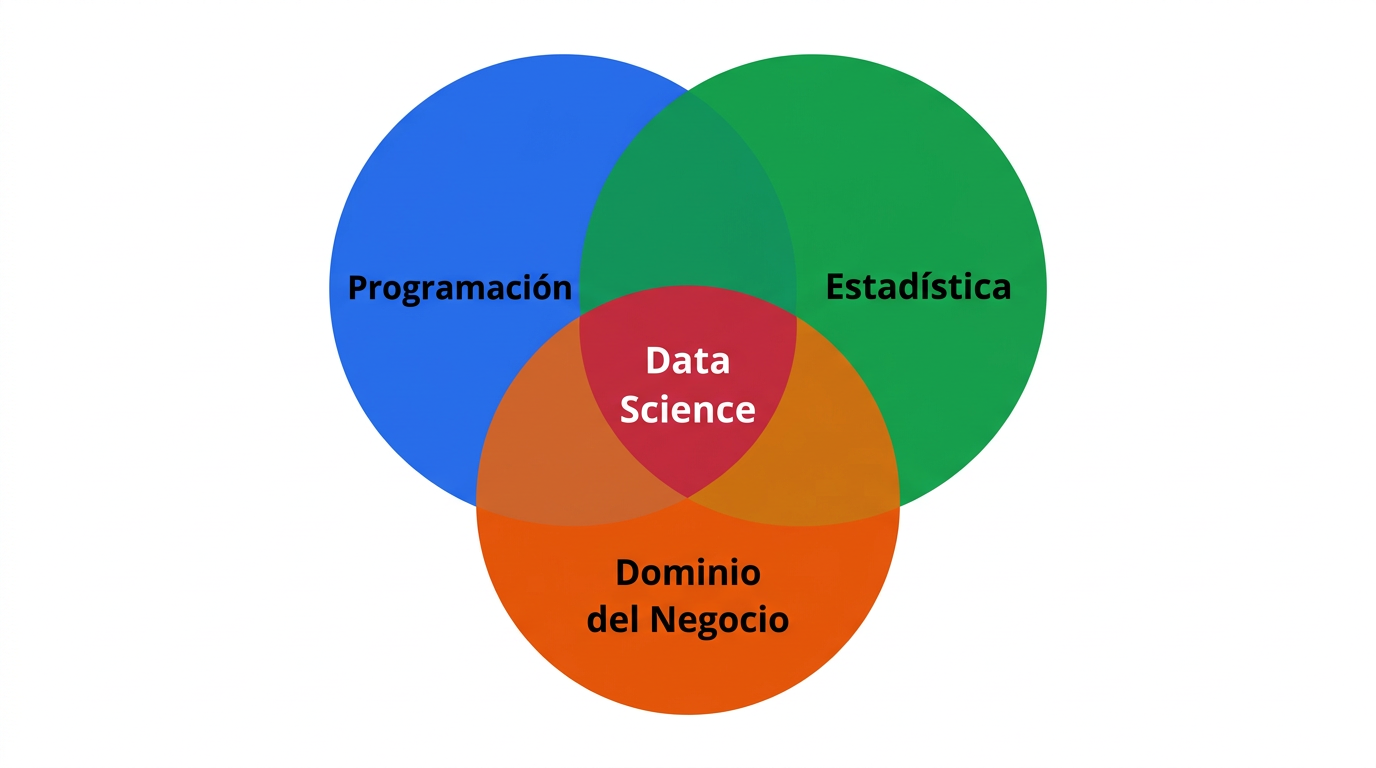
\includegraphics[width=\textwidth]{data_science_venn.png}
      \end{center}
    \end{column}

    \begin{column}{0.48\textwidth}
      {\footnotesize\color{arcaDark}\itshape
        ``Persona que sabe más de estadística que cualquier
        programador, y más de programación que cualquier
        estadístico.''}

      \vspace{4pt}
      {\scriptsize\color{textMuted}
        --- Josh Wills, Director of Data Engineering, Slack}

      \vspace{10pt}
      {\scriptsize\color{textMuted}
      \begin{itemize}\setlength{\itemsep}{4pt}
        \item[{\color{arcaRed}\scriptsize\faArrowRight}]
          Ustedes ya tienen el \textbf{dominio} (Arca Continental).
        \item[{\color{arcaRed}\scriptsize\faArrowRight}]
          Ya aprendieron \textbf{programación} (Python, pandas).
        \item[{\color{arcaRed}\scriptsize\faArrowRight}]
          Hoy empezamos la \textbf{estadística}.
      \end{itemize}
      }
    \end{column}
  \end{columns}
\end{frame}

% ── EDA INTRO ────────────────────────────────────────────────────────────────
\begin{frame}{Hoy: Conoce tus Datos (EDA)}
  \vspace{-4pt}
  {\footnotesize
    Lo que vamos a hacer tiene un nombre formal:
    \textbf{Análisis Exploratorio de Datos (EDA)}.
    Es lo primero que hace un data scientist al recibir un dataset.}

  \vspace{6pt}
  \begin{center}
  \begin{tikzpicture}[
    node distance=0.6cm,
    step/.style={rectangle, rounded corners=3pt, draw=#1, fill=#1!10,
                 font=\scriptsize\bfseries\color{#1}, minimum height=0.6cm,
                 minimum width=2.5cm, align=center},
    arr/.style={-{Stealth[length=3pt]}, line width=0.6pt, textMuted}
  ]
    \node[step=dikwData] (s1) {1. Estructura};
    \node[step=dikwInfo, right=of s1] (s2) {2. Tipos de dato};
    \node[step=dikwKnow, right=of s2] (s3) {3. Datos faltantes};
    \node[step=dikwWis, right=of s3] (s4) {4. Visualizar};

    \draw[arr] (s1) -- (s2);
    \draw[arr] (s2) -- (s3);
    \draw[arr] (s3) -- (s4);

    \node[font=\tiny\color{textMuted}, below=0.2cm of s1] {DataFrame vs Series};
    \node[font=\tiny\color{textMuted}, below=0.2cm of s2] {int, float, object\ldots};
    \node[font=\tiny\color{textMuted}, below=0.2cm of s3] {NaN, fillna, dropna};
    \node[font=\tiny\color{textMuted}, below=0.2cm of s4] {Histograma, Boxplot};
  \end{tikzpicture}
  \end{center}

  \vspace{4pt}
  {\scriptsize\color{textMuted}
    \faLightbulb\ Antes de calcular, antes de predecir:
    \textbf{entender qué tienes}.}
\end{frame}

% ── RECAP ────────────────────────────────────────────────────────────────────
\begin{frame}{¿Dónde Quedamos?}
  \vspace{-4pt}
  {\small\color{arcaDark}\bfseries Módulo 1 --- lo que ya dominan:}
  \vspace{4pt}
  {\footnotesize
  \begin{itemize}\setlength{\itemsep}{4pt}
    \item[{\color{codeGreen}\faCheckCircle}]
      Python: variables, control de flujo, funciones, \texttt{try/except}.
    \item[{\color{codeGreen}\faCheckCircle}]
      pandas: \texttt{read\_csv}, filtrar, \texttt{groupby}, \texttt{agg}, \texttt{apply}.
    \item[{\color{codeGreen}\faCheckCircle}]
      Importar módulos, exportar CSV.
  \end{itemize}
  }
  \vspace{8pt}
  {\small\color{arcaRed}\bfseries Hoy agregamos:}
  \vspace{4pt}
  {\footnotesize
  \begin{itemize}\setlength{\itemsep}{4pt}
    \item[{\color{arcaRed}\faArrowRight}]
      DataFrame vs Series --- la estructura de pandas.
    \item[{\color{arcaRed}\faArrowRight}]
      Tipos de dato: numérico vs categórico y por qué importa.
    \item[{\color{arcaRed}\faArrowRight}]
      Datos faltantes: detectar y tratar (media, mediana, moda).
    \item[{\color{arcaRed}\faArrowRight}]
      Primer histograma y boxplot con seaborn.
  \end{itemize}
  }
\end{frame}

% ── DATASET ──────────────────────────────────────────────────────────────────
\begin{frame}[fragile,shrink=28]{Nuestro Dataset: Supermarket Sales}
  \vspace{-6pt}
  {\footnotesize
    1\,000 transacciones de 3 sucursales de un supermercado.
    \textbf{Tiene datos faltantes} --- como pasa en la vida real.}

  \vspace{4pt}
  \begin{pyblock}
import pandas as pd

url = ("https://raw.githubusercontent.com/cmosquerat/"
       "arca-diplomado/main/clase-08/supermarket_sales.csv")
df = pd.read_csv(url)
print(f"Forma: {df.shape}")
print(f"NaN totales: {df.isna().sum().sum()}")
df.head(3)
  \end{pyblock}

  \vspace{4pt}
  {\scriptsize\color{textMuted}
  \begin{itemize}\setlength{\itemsep}{2pt}
    \item[{\color{arcaRed}\scriptsize\faArrowRight}]
      Columnas: Branch, City, Product line, Total, Payment, Rating\ldots
    \item[{\color{codeOrange}\scriptsize\faExclamationTriangle}]
      Rating, Payment y Total tienen valores faltantes. Los trataremos hoy.
  \end{itemize}
  }
\end{frame}

% =============================================================================
%  SECCIÓN 1: DATAFRAME VS SERIES
% =============================================================================
\sectionframe{DataFrame vs Series}{La estructura fundamental de pandas}

\begin{frame}{DataFrame vs Series --- Visualmente}
  \vspace{-4pt}
  \begin{columns}[c]
    \begin{column}{0.55\textwidth}
      {\small\bfseries\color{arcaDark} DataFrame = Tabla (2D)}
      \vspace{4pt}

      {\scriptsize
      \begin{tabular}{@{}c|lrr@{}}
        \rowcolor{arcaRed}
        \textcolor{white}{\bfseries} &
        \textcolor{white}{\bfseries Branch} &
        \textcolor{white}{\bfseries Total} &
        \textcolor{white}{\bfseries Rating} \\
        \midrule
        \rowcolor{arcaGray} \textbf{0} & A & 337.9 & 9.1 \\
        \textbf{1} & C & 489.0 & 7.2 \\
        \rowcolor{arcaGray} \textbf{2} & A & 205.2 & 8.4 \\
      \end{tabular}
      }

      \vspace{4pt}
      {\scriptsize\color{textMuted}
        Filas $\times$ Columnas = \textbf{2 dimensiones}.}
    \end{column}

    \begin{column}{0.05\textwidth}
      \centering
      {\color{textMuted}\Large$\to$}
    \end{column}

    \begin{column}{0.35\textwidth}
      {\small\bfseries\color{codeBlue} Series = Columna (1D)}
      \vspace{4pt}

      {\scriptsize
      \begin{tabular}{@{}c|r@{}}
        \rowcolor{codeBlue}
        \textcolor{white}{\bfseries} &
        \textcolor{white}{\bfseries Total} \\
        \midrule
        \rowcolor{arcaGray} \textbf{0} & 337.9 \\
        \textbf{1} & 489.0 \\
        \rowcolor{arcaGray} \textbf{2} & 205.2 \\
      \end{tabular}
      }

      \vspace{4pt}
      {\scriptsize\color{textMuted}
        1 columna = \textbf{1 dimensión}.}
    \end{column}
  \end{columns}

  \vspace{10pt}
  {\scriptsize\color{textMuted}
  \begin{itemize}\setlength{\itemsep}{3pt}
    \item[{\color{arcaRed}\scriptsize\faArrowRight}]
      \texttt{df["Total"]} $\to$ \textbf{Series}. \quad
      \texttt{df[["Total","Rating"]]} $\to$ \textbf{DataFrame}.
    \item[{\color{arcaRed}\scriptsize\faLightbulb}]
      Un DataFrame es un \textbf{diccionario de Series} que comparten el mismo índice.
  \end{itemize}
  }
\end{frame}

\begin{frame}[fragile,shrink=28]{DataFrame vs Series --- En Código}
  \vspace{-6pt}
  \begin{columns}[T]
    \begin{column}{0.48\textwidth}
      {\scriptsize\color{codeBlue}\bfseries Series (una columna):}
      \begin{pyblock}[minted options={fontsize=\scriptsize, breaklines}]
s = df["Total"]
print("Tipo:", type(s).__name__)
print("Forma:", s.shape)
print(s.head(3))
      \end{pyblock}
      \vspace{-2pt}
      \begin{outputblock}[minted options={fontsize=\scriptsize, breaklines}]
Tipo: Series
Forma: (1000,)
0    337.9
1    489.0
2    205.2
      \end{outputblock}
    \end{column}

    \begin{column}{0.48\textwidth}
      {\scriptsize\color{arcaDark}\bfseries DataFrame (varias):}
      \begin{pyblock}[minted options={fontsize=\scriptsize, breaklines}]
sub = df[["Branch", "Total"]]
print("Tipo:", type(sub).__name__)
print("Forma:", sub.shape)
sub.head(3)
      \end{pyblock}
      \vspace{-2pt}
      \begin{outputblock}[minted options={fontsize=\scriptsize, breaklines}]
Tipo: DataFrame
Forma: (1000, 2)
  Branch  Total
0      A  337.9
1      C  489.0
      \end{outputblock}
    \end{column}
  \end{columns}
\end{frame}

% =============================================================================
%  SECCIÓN 2: TIPOS DE DATO
% =============================================================================
\sectionframe{Tipos de Dato en pandas}{Por qué importan más de lo que crees}

\begin{frame}{Los Tipos de Dato de pandas}
  \vspace{-4pt}
  {\footnotesize
    Cada columna tiene un tipo. Si el tipo está mal,
    las operaciones fallan \textbf{silenciosamente}.}

  \vspace{6pt}
  {\small
  \begin{tabular}{@{}llll@{}}
    \toprule
    \textbf{dtype} & \textbf{Qué guarda} & \textbf{Ejemplo} & \textbf{Operaciones} \\
    \midrule
    \texttt{int64}     & Enteros    & 30, 150    & Suma, media \\
    \texttt{float64}   & Decimales  & 12.50, 3.14 & Suma, media \\
    \texttt{object}    & Texto      & ``Ana'', ``Norte'' & Conteo, filtro \\
    \texttt{bool}      & Verdadero/Falso & True, False & Filtro \\
    \texttt{datetime64} & Fechas    & 2026-03-25 & Rango, mes \\
    \texttt{category}  & Categorías & ``A'', ``B'', ``C'' & Ahorra memoria \\
    \bottomrule
  \end{tabular}
  }

  \vspace{6pt}
  {\scriptsize\color{textMuted}
    \faExclamationTriangle\ Si una columna de números aparece como
    \texttt{object}, \textbf{no puedes sumar}.}
\end{frame}

% ── POR QUÉ IMPORTA NUMÉRICO VS CATEGÓRICO ──────────────────────────────────
\begin{frame}{¿Por Qué Importa Numérico vs Categórico?}
  \vspace{-4pt}
  \begin{center}
  \begin{tikzpicture}[
    scale=0.85, transform shape,
    box/.style={rectangle, rounded corners=4pt, draw=#1, fill=#1!8,
                minimum width=4.8cm, minimum height=0.6cm,
                font=\scriptsize\bfseries\color{#1}, align=center},
    op/.style={font=\tiny\color{textMuted}, text width=4.5cm, align=left},
    arr/.style={-{Stealth[length=3pt]}, line width=0.6pt}
  ]
    % Numérico
    \node[box=codeBlue] (num) at (-3.5, 2.5) {Numérico (int64, float64)};
    \node[op, below=0.15cm of num] (numops) {%
      \faCheckCircle\ Media, mediana, suma, std\\
      \faCheckCircle\ Histograma, boxplot, scatter\\
      \faCheckCircle\ Correlación, regresión};

    % Categórico
    \node[box=codeOrange] (cat) at (3.5, 2.5) {Categórico (object, category)};
    \node[op, below=0.15cm of cat] (catops) {%
      \faCheckCircle\ Conteo, frecuencia, moda\\
      \faCheckCircle\ Gráfico de barras, pie chart\\
      \faCheckCircle\ Agrupación (groupby)};

    % Danger zone
    \node[rectangle, rounded corners=3pt, draw=arcaRed, fill=arcaRed!8,
          minimum width=10cm, minimum height=0.6cm,
          font=\scriptsize\bfseries\color{arcaRed}, align=center]
      (danger) at (0, -0.2)
      {\faExclamationTriangle\quad Si el tipo está mal, el análisis está mal};

    \node[op, text width=10cm, align=center, below=0.1cm of danger] {%
      \texttt{df["precio"].sum()} con \texttt{object}
      $\to$ \textbf{concatena textos} en vez de sumar\\[2pt]
      \texttt{df["sucursal"].mean()} con \texttt{int64}
      $\to$ \textbf{promedio sin sentido}};
  \end{tikzpicture}
  \end{center}
\end{frame}

\begin{frame}[fragile,shrink=28]{Inspeccionar Tipos: \texttt{.dtypes} e \texttt{.info()}}
  \vspace{-6pt}
  \begin{pyblock}
print(df.dtypes)
  \end{pyblock}

  \vspace{4pt}
  {\footnotesize\color{arcaDark}\bfseries ¿Qué buscar?}
  \vspace{2pt}
  {\scriptsize\color{textMuted}
  \begin{itemize}\setlength{\itemsep}{3pt}
    \item[{\color{codeGreen}\scriptsize\faCheckCircle}]
      \texttt{Total}, \texttt{Unit price} $\to$ \texttt{float64} --- correcto.
    \item[{\color{codeOrange}\scriptsize\faExclamationTriangle}]
      \texttt{Date} $\to$ \texttt{object} --- debería ser \texttt{datetime64}.
    \item[{\color{arcaRed}\scriptsize\faArrowRight}]
      \texttt{df.info()} muestra tipos + cantidad de no-nulos en un resumen.
  \end{itemize}
  }
\end{frame}

\begin{frame}[fragile,shrink=28]{Convertir Tipos (I): Fechas y Categorías}
  \vspace{-6pt}
  {\footnotesize\color{arcaDark}\bfseries
    Las fechas suelen llegar como texto (\texttt{object}).
    Hay que convertirlas para operar con ellas:}

  \vspace{4pt}
  \begin{pyblock}
# Ejemplo: una Serie con fechas como texto
fechas = pd.Series(["2025-01-15", "2025-02-20",
                     "2025-03-10"])
print("Tipo original:", fechas.dtype)

# Convertir a datetime
fechas_dt = pd.to_datetime(fechas)
print("Tipo nuevo:   ", fechas_dt.dtype)

# Ahora puedes extraer componentes
print("Mes:", fechas_dt.dt.month.tolist())
print("Dia:", fechas_dt.dt.day_name().tolist())
  \end{pyblock}

  \vspace{4pt}
  {\scriptsize\color{textMuted}
  \begin{itemize}\setlength{\itemsep}{3pt}
    \item[{\color{arcaRed}\scriptsize\faArrowRight}]
      \texttt{pd.to\_datetime()} para convertir texto a fecha.
    \item[{\color{arcaRed}\scriptsize\faArrowRight}]
      \texttt{.dt.month}, \texttt{.dt.day\_name()} para extraer componentes.
    \item[{\color{arcaRed}\scriptsize\faArrowRight}]
      \texttt{.astype("category")} para ahorrar memoria en columnas repetitivas.
  \end{itemize}
  }
\end{frame}

\begin{frame}[fragile,shrink=28]{Convertir Tipos (II): \texttt{pd.to\_numeric()} y \texttt{.astype()}}
  \vspace{-6pt}
  {\footnotesize\color{arcaDark}\bfseries
    A veces una columna numérica llega como texto (``object''):}

  \vspace{4pt}
  \begin{pyblock}
import numpy as np
s = pd.Series(["10", "20", "treinta", "40"])
print("Tipo original:", s.dtype)

# to_numeric con errors="coerce": invalidos -> NaN
s_num = pd.to_numeric(s, errors="coerce")
print(s_num)
print("Tipo:", s_num.dtype)
  \end{pyblock}

  \vspace{4pt}
  {\scriptsize\color{textMuted}
  \begin{itemize}\setlength{\itemsep}{3pt}
    \item[{\color{arcaRed}\scriptsize\faArrowRight}]
      \texttt{errors="coerce"}: lo que no se puede convertir $\to$ \texttt{NaN}.
    \item[{\color{arcaRed}\scriptsize\faArrowRight}]
      \texttt{.astype(int)} para forzar un tipo (falla si hay valores inválidos).
  \end{itemize}
  }
\end{frame}

% ── RESUMEN CONVERSIONES ─────────────────────────────────────────────────────
\begin{frame}{Resumen: Herramientas de Conversión}
  \vspace{-4pt}
  {\small
  \begin{tabular}{@{}lll@{}}
    \toprule
    \textbf{Función} & \textbf{Cuándo usarla} & \textbf{Manejo de errores} \\
    \midrule
    \texttt{pd.to\_datetime()} & Texto $\to$ fecha & \texttt{errors="coerce"} \\
    \texttt{pd.to\_numeric()}  & Texto $\to$ número & \texttt{errors="coerce"} \\
    \texttt{.astype(int)}     & Cambio explícito & Falla si hay inválidos \\
    \texttt{.astype("category")} & Reducir memoria & Siempre funciona \\
    \texttt{.astype(str)}     & Número $\to$ texto & Siempre funciona \\
    \bottomrule
  \end{tabular}
  }

  \vspace{8pt}
  {\scriptsize\color{textMuted}
    \faLightbulb\ \texttt{errors="coerce"} es tu aliado: convierte lo que puede
    y marca lo demás como \texttt{NaN} para que lo revises después.}
\end{frame}

\begin{frame}[fragile,shrink=28]{Numérico vs Categórico: \texttt{select\_dtypes()}}
  \vspace{-6pt}
  {\footnotesize
    Separar columnas por tipo es fundamental para el análisis.}

  \vspace{4pt}
  \begin{pyblock}
# Solo columnas numericas
num = df.select_dtypes(include="number")
print("Numericas:", list(num.columns))

# Solo columnas de texto
cat = df.select_dtypes(include="object")
print("Categoricas:", list(cat.columns))
  \end{pyblock}

  \vspace{4pt}
  {\scriptsize\color{textMuted}
  \begin{itemize}\setlength{\itemsep}{3pt}
    \item[{\color{arcaRed}\scriptsize\faArrowRight}]
      Numéricas $\to$ media, suma, histograma.
    \item[{\color{arcaRed}\scriptsize\faArrowRight}]
      Categóricas $\to$ conteo, \texttt{value\_counts()}, gráfico de barras.
  \end{itemize}
  }
\end{frame}

\begin{frame}[fragile,shrink=28]{Describe: Resumen por Tipo}
  \vspace{-6pt}
  \begin{columns}[T]
    \begin{column}{0.48\textwidth}
      {\scriptsize\color{arcaDark}\bfseries Numéricas:}
      \begin{pyblock}[minted options={fontsize=\scriptsize, breaklines}]
print(df.describe())
      \end{pyblock}
      \vspace{2pt}
      {\scriptsize\color{textMuted}
        count, mean, std, min, 25\%, 50\%, 75\%, max.}
    \end{column}

    \begin{column}{0.48\textwidth}
      {\scriptsize\color{arcaDark}\bfseries Categóricas:}
      \begin{pyblock}[minted options={fontsize=\scriptsize, breaklines}]
print(df.describe(include="object"))
      \end{pyblock}
      \vspace{2pt}
      {\scriptsize\color{textMuted}
        count, unique, top (más frecuente), freq.}
    \end{column}
  \end{columns}

  \vspace{6pt}
  {\scriptsize\color{textMuted}
    \faLightbulb\ \texttt{.describe()} sin argumentos solo muestra numéricas.
    Con \texttt{include="object"} muestra las categóricas.}
\end{frame}

% ── EJERCICIO 1 ──────────────────────────────────────────────────────────────
\begin{frame}[fragile,shrink=28]{Ejercicio 1: Inspecciona el Dataset \hfill
    {\normalsize\color{arcaRed}\faClock\ 5 min}}
  \vspace{-6pt}
  {\footnotesize\color{arcaDark}\bfseries
    Sobre el dataset \texttt{df} que ya cargamos, respondan:}

  \vspace{4pt}
  \begin{pyblock}
# 1. Cuantas columnas numericas tiene?
#    Pista: select_dtypes(include="number")

# 2. Cuantas categoricas?
#    Pista: select_dtypes(include="object")

# 3. Que tipo tiene la columna "Date"?
#    Que tipo DEBERIA tener?

# 4. Convierte "Date" a datetime
#    Pista: pd.to_datetime()
  \end{pyblock}

  \vspace{4pt}
  {\scriptsize\color{textMuted}
  \begin{itemize}\setlength{\itemsep}{3pt}
    \item[{\color{arcaRed}\scriptsize\faLightbulb}]
      \texttt{df.dtypes} para ver todos los tipos.
    \item[{\color{arcaRed}\scriptsize\faLightbulb}]
      \texttt{len(df.select\_dtypes(include="number").columns)} para contar.
  \end{itemize}
  }
\end{frame}

% =============================================================================
%  SECCIÓN 3: DATOS FALTANTES
% =============================================================================
\sectionframe{Datos Faltantes: NaN}{El problema más común en datos reales}

\begin{frame}{¿Qué Es NaN?}
  \vspace{-4pt}
  \begin{center}
  \begin{tikzpicture}[
    box/.style={rectangle, rounded corners=3pt, minimum width=3cm,
                minimum height=0.6cm, font=\scriptsize\bfseries, align=center},
    arr/.style={-{Stealth[length=3pt]}, line width=0.6pt, textMuted}
  ]
    \node[box, draw=arcaRed, fill=arcaRed!10, text=arcaRed] (nan) at (0,0)
      {NaN = Not a Number};
    \node[box, draw=codeOrange, fill=codeOrange!10, text=codeOrange] (no0) at (5,0.8)
      {NaN $\neq$ 0};
    \node[box, draw=codeOrange, fill=codeOrange!10, text=codeOrange] (nostr) at (5,0)
      {NaN $\neq$ ``''};
    \node[box, draw=codeOrange, fill=codeOrange!10, text=codeOrange] (noF) at (5,-0.8)
      {NaN $\neq$ False};

    \draw[arr] (nan) -- (no0);
    \draw[arr] (nan) -- (nostr);
    \draw[arr] (nan) -- (noF);
  \end{tikzpicture}
  \end{center}

  \vspace{4pt}
  {\footnotesize
    NaN significa \textbf{``no hay dato''}.
    Alguien no llenó el campo, el sensor falló, o el dato se perdió.}

  \vspace{6pt}
  {\scriptsize\color{textMuted}
  \begin{itemize}\setlength{\itemsep}{3pt}
    \item[{\color{codeOrange}\scriptsize\faExclamationTriangle}]
      Si calculas la media con NaN, pandas lo \textbf{ignora silenciosamente}.
    \item[{\color{codeOrange}\scriptsize\faExclamationTriangle}]
      Si filtras, las filas con NaN pueden \textbf{desaparecer} sin aviso.
    \item[{\color{arcaRed}\scriptsize\faArrowRight}]
      Siempre hay que \textbf{detectar y decidir} qué hacer con ellos.
  \end{itemize}
  }
\end{frame}

\begin{frame}[fragile,shrink=28]{Detectar NaN en Nuestro Dataset}
  \vspace{-6pt}
  \begin{pyblock}
print("=== NaN por columna ===")
print(df.isna().sum())

print("\n=== % faltante ===")
pct = (df.isna().sum() / len(df) * 100).round(1)
print(pct[pct > 0])
  \end{pyblock}

  \vspace{2pt}
  \begin{outputblock}[minted options={fontsize=\scriptsize, breaklines}]
Rating          35    (3.5%)
Payment         20    (2.0%)
Total           15    (1.5%)
Tax 5%          15    (1.5%)
gross income    15    (1.5%)
  \end{outputblock}
\end{frame}

% ── MEDIA VS MEDIANA VS MODA ────────────────────────────────────────────────
\begin{frame}{¿Cuándo Usar Media, Mediana o Moda?}
  \vspace{-4pt}
  \begin{center}
  \begin{tikzpicture}[
    scale=0.85, transform shape,
    card/.style={rectangle, rounded corners=4pt, draw=#1, fill=#1!6,
                 minimum width=3.8cm, minimum height=3.6cm,
                 align=center},
    ttl/.style={font=\small\bfseries\color{#1}},
    desc/.style={font=\tiny\color{textDark}, text width=3.2cm, align=left},
  ]
    % Media
    \node[card=codeBlue] (med) at (0,0) {};
    \node[ttl=codeBlue, above] at (0, 0.8) {Media (promedio)};
    \node[desc] at (0, 0.1) {%
      \textbf{Cuándo:} Distribución simétrica,
      sin outliers extremos.\\[3pt]
      \textbf{Ejemplo:} Calificación de
      productos (Rating).\\[3pt]
      \textbf{Código:}\\
      \texttt{df["col"].mean()}};

    % Mediana
    \node[card=codeGreen] (mdn) at (4.5,0) {};
    \node[ttl=codeGreen, above] at (4.5, 0.8) {Mediana};
    \node[desc] at (4.5, 0.1) {%
      \textbf{Cuándo:} Hay outliers o
      distribución sesgada.\\[3pt]
      \textbf{Ejemplo:} Salarios, montos
      de venta (Total).\\[3pt]
      \textbf{Código:}\\
      \texttt{df["col"].median()}};

    % Moda
    \node[card=codeOrange] (mod) at (9.0,0) {};
    \node[ttl=codeOrange, above] at (9.0, 0.8) {Moda};
    \node[desc] at (9.0, 0.1) {%
      \textbf{Cuándo:} Datos categóricos
      (texto), o discretos.\\[3pt]
      \textbf{Ejemplo:} Método de pago,
      ciudad, sucursal.\\[3pt]
      \textbf{Código:}\\
      \texttt{df["col"].mode()[0]}};
  \end{tikzpicture}
  \end{center}

  \vspace{2pt}
  {\scriptsize\color{textMuted}
    \faLightbulb\ \textbf{Regla de oro:} Si hay outliers $\to$ mediana.
    Si es texto $\to$ moda. Si es simétrica $\to$ media.}
\end{frame}

\begin{frame}{Estrategias para Tratar NaN}
  \vspace{-4pt}
  \begin{center}
  \begin{tikzpicture}[
    node distance=0.4cm,
    strat/.style={rectangle, rounded corners=3pt, draw=#1, fill=#1!8,
                  minimum width=4.8cm, minimum height=0.55cm,
                  font=\scriptsize\bfseries\color{#1}, align=center},
    when/.style={font=\tiny\color{textMuted}, text width=5.5cm, align=left}
  ]
    \node[strat=codeGreen] (drop) at (0,0)
      {\faTrash\hspace{4pt}dropna() --- Eliminar filas};
    \node[when, right=0.3cm of drop]
      {Pocos NaN ($<$ 5\%). Perder filas no importa.};

    \node[strat=codeBlue, below=of drop] (fmdn)
      {\faChartBar\hspace{4pt}fillna(mediana) --- Con outliers};
    \node[when, right=0.3cm of fmdn]
      {Columna numérica sesgada: ventas, salarios, montos.};

    \node[strat=dikwInfo, below=of fmdn] (fmea)
      {\faChartLine\hspace{4pt}fillna(media) --- Sin outliers};
    \node[when, right=0.3cm of fmea]
      {Columna numérica simétrica: rating, temperatura.};

    \node[strat=dikwKnow, below=of fmea] (fcat)
      {\faFont\hspace{4pt}fillna(moda) --- Categórica};
    \node[when, right=0.3cm of fcat]
      {Columna de texto: método de pago, ciudad.};

    \node[strat=arcaRed, below=of fcat] (no)
      {\faTimesCircle\hspace{4pt}fillna(0) --- Casi nunca};
    \node[when, right=0.3cm of no]
      {Solo si 0 tiene significado real en el contexto.};
  \end{tikzpicture}
  \end{center}
\end{frame}

\begin{frame}[fragile,shrink=28]{Tratar NaN --- Nuestro Dataset}
  \vspace{-6pt}
  {\footnotesize\color{arcaDark}\bfseries Apliquemos las estrategias a nuestros datos reales:}

  \vspace{4pt}
  \begin{pyblock}
# Total tiene outliers -> mediana
df["Total"] = df["Total"].fillna(df["Total"].median())
df["Tax 5%"] = df["Tax 5%"].fillna(df["Tax 5%"].median())
df["gross income"] = df["gross income"].fillna(
    df["gross income"].median())

# Rating es simetrica -> media
df["Rating"] = df["Rating"].fillna(df["Rating"].mean())

# Payment es categorica -> moda
df["Payment"] = df["Payment"].fillna(df["Payment"].mode()[0])

print("NaN restantes:", df.isna().sum().sum())
  \end{pyblock}

  \vspace{2pt}
  \begin{outputblock}[minted options={fontsize=\scriptsize, breaklines}]
NaN restantes: 0
  \end{outputblock}
\end{frame}

\begin{frame}[fragile,shrink=28]{Ejercicio 2: Limpia el Dataset \hfill
    {\normalsize\color{arcaRed}\faClock\ 5 min}}
  \vspace{-6pt}
  {\footnotesize\color{arcaDark}\bfseries
    Nuestro dataset tiene NaN reales. Resuélvanlos:}

  \vspace{4pt}
  \begin{pyblock}
# Recarga el dataset
url = ("https://raw.githubusercontent.com/cmosquerat/"
       "arca-diplomado/main/clase-08/supermarket_sales.csv")
df = pd.read_csv(url)

# 1. Cuantos NaN hay por columna?

# 2. Que % representan? (sobre 1000 filas)

# 3. Rellena "Rating" -- es simetrica, que usar?

# 4. Rellena "Payment" -- es texto, que usar?

# 5. Rellena "Total" -- tiene outliers, que usar?

# 6. Verifica: df.isna().sum().sum() == 0?
  \end{pyblock}

  \vspace{4pt}
  {\scriptsize\color{textMuted}
    \faLightbulb\ Rating $\to$ \texttt{.mean()}, \quad
    Payment $\to$ \texttt{.mode()[0]}, \quad
    Total $\to$ \texttt{.median()}}
\end{frame}

% =============================================================================
%  SECCIÓN 4: PRIMER HISTOGRAMA Y BOXPLOT
% =============================================================================
\sectionframe{Visualizar para Entender}{Histograma y boxplot con seaborn}

\begin{frame}[fragile,shrink=28]{seaborn: Gráficas en Una Línea}
  \vspace{-6pt}
  {\footnotesize
    seaborn se construye sobre matplotlib.
    Una línea, resultado profesional.}

  \vspace{4pt}
  \begin{pyblock}
import seaborn as sns
import matplotlib.pyplot as plt

# Histograma: distribucion de Total
sns.histplot(df["Total"], bins=20, color="#C82B40")
plt.title("Distribucion del Total de Venta")
plt.xlabel("Total ($)")
plt.show()
  \end{pyblock}

  \vspace{4pt}
  {\scriptsize\color{textMuted}
  \begin{itemize}\setlength{\itemsep}{3pt}
    \item[{\color{arcaRed}\scriptsize\faArrowRight}]
      El histograma responde: ¿cómo se \textbf{distribuyen} los valores?
    \item[{\color{arcaRed}\scriptsize\faLightbulb}]
      ¿Se acumulan a la izquierda? ¿Hay picos? ¿Hay colas largas?
  \end{itemize}
  }
\end{frame}

\begin{frame}[fragile,shrink=28]{Boxplot: Dispersión y Outliers}
  \vspace{-6pt}
  {\footnotesize
    El boxplot muestra \textbf{mediana, cuartiles y outliers} en un gráfico.}

  \vspace{4pt}
  \begin{pyblock}
sns.boxplot(data=df, x="Product line", y="Total",
            palette="Set2")
plt.title("Total por Linea de Producto")
plt.xticks(rotation=45)
plt.tight_layout()
plt.show()
  \end{pyblock}

  \vspace{4pt}
  {\scriptsize\color{textMuted}
  \begin{itemize}\setlength{\itemsep}{3pt}
    \item[{\color{arcaRed}\scriptsize\faArrowRight}]
      La caja = 50\% central de los datos (Q1 a Q3).
    \item[{\color{arcaRed}\scriptsize\faArrowRight}]
      La línea dentro = mediana. Puntos fuera = \textbf{outliers}.
  \end{itemize}
  }
\end{frame}

\begin{frame}{Anatomía del Boxplot}
  \vspace{-4pt}
  \begin{center}
    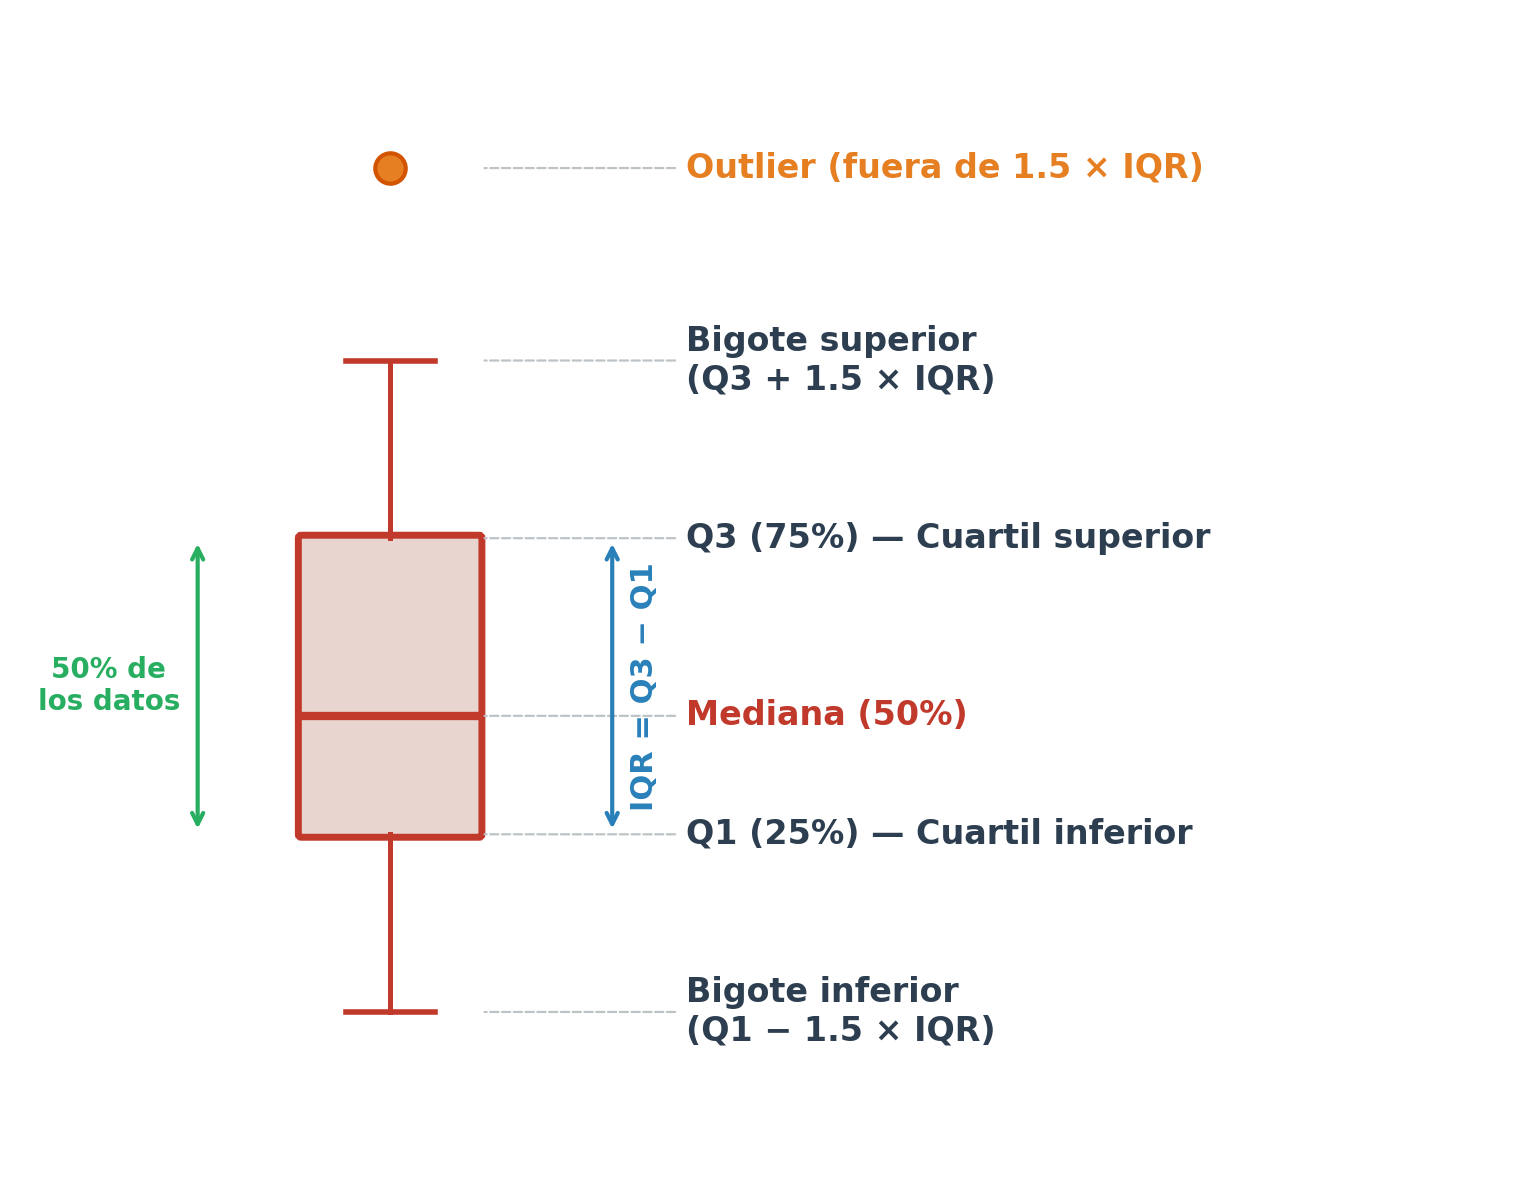
\includegraphics[width=0.85\textwidth]{boxplot_anatomia.png}
  \end{center}
\end{frame}

\begin{frame}[fragile,shrink=28]{Práctica: Visualizar el Dataset \hfill
    {\normalsize\color{arcaRed}\faClock\ 10 min}}
  \vspace{-6pt}
  \begin{pyblock}
import seaborn as sns
import matplotlib.pyplot as plt

# 1. Histograma de Rating

# 2. Boxplot de Total por Branch

# 3. Boxplot de Rating por Gender

# 4. Que historia cuentan los graficos?
  \end{pyblock}

  \vspace{6pt}
  {\scriptsize\color{textMuted}
  \begin{itemize}\setlength{\itemsep}{3pt}
    \item[{\color{arcaRed}\scriptsize\faLightbulb}]
      \texttt{sns.histplot(df["col"], bins=20)}.
    \item[{\color{arcaRed}\scriptsize\faLightbulb}]
      \texttt{sns.boxplot(data=df, x="cat", y="num")}.
    \item[{\color{arcaRed}\scriptsize\faLightbulb}]
      Busquen: ¿Hay outliers? ¿Las distribuciones son iguales entre grupos?
  \end{itemize}
  }
\end{frame}

% =============================================================================
%  CIERRE
% =============================================================================
\sectionframe{Cierre}{Lo que logramos hoy}

\begin{frame}{Lo que Aprendimos Hoy}
  \vspace{-4pt}
  \begin{columns}[T]
    \begin{column}{0.52\textwidth}
      {\footnotesize
      \begin{itemize}\setlength{\itemsep}{4pt}
        \item[{\color{codeGreen}\faCheckCircle}]
          DIKW: Dato $\to$ Información $\to$ Conocimiento.
        \item[{\color{codeGreen}\faCheckCircle}]
          DataFrame (2D) vs Series (1D).
        \item[{\color{codeGreen}\faCheckCircle}]
          Tipos de dato: numérico vs categórico.
        \item[{\color{codeGreen}\faCheckCircle}]
          Conversión: \texttt{to\_datetime}, \texttt{to\_numeric}.
      \end{itemize}
      }
    \end{column}

    \begin{column}{0.44\textwidth}
      {\footnotesize
      \begin{itemize}\setlength{\itemsep}{4pt}
        \item[{\color{codeGreen}\faCheckCircle}]
          NaN: detectar con \texttt{isna()}.
        \item[{\color{codeGreen}\faCheckCircle}]
          Rellenar: media, mediana o moda.
        \item[{\color{codeGreen}\faCheckCircle}]
          Histograma con seaborn.
        \item[{\color{codeGreen}\faCheckCircle}]
          Boxplot y anatomía.
      \end{itemize}
      }
    \end{column}
  \end{columns}

  \vspace{6pt}
  {\small\color{arcaDark}\bfseries Próxima clase (viernes 27):}
  \vspace{2pt}
  {\footnotesize
  \begin{itemize}\setlength{\itemsep}{2pt}
    \item[{\color{arcaRed}\faArrowRight}]
      Estadística descriptiva: media, mediana, moda en profundidad.
    \item[{\color{arcaRed}\faArrowRight}]
      Dispersión: desviación estándar, varianza, IQR.
    \item[{\color{arcaRed}\faArrowRight}]
      Outliers: cómo detectarlos y qué hacer con ellos.
  \end{itemize}
  }
\end{frame}

% ── QR ENCUESTA ──────────────────────────────────────────────────────────────
{
\setbeamertemplate{headline}{}
\setbeamertemplate{footline}{}
\begin{frame}[plain, noframenumbering]
  \begin{tikzpicture}[remember picture, overlay]
    \fill[arcaDark] (current page.south west) rectangle (current page.north east);
  \end{tikzpicture}
  \vspace{1cm}
  \begin{center}
    {\Huge\bfseries\color{white} ¿Cómo estuvo la clase?\par}
    \vspace{0.6cm}
    
\includegraphics[width=4cm]{qr_encuesta.jpg}
    \vspace{0.4cm}
    {\large\color{white!80} Escaneen el QR para la encuesta rápida\par}
  \end{center}
\end{frame}
}

\end{document}
